\section{Minimum Cost Steiner Trees} \label{sec:5}

\subsection{Minimum Steiner Tree Problem}
Given an (undirected) graph $G = (V, E)$, edge costs $c_e \geq 0$ for all 
$e \in E$, and {\bf terminals} $T \subseteq V$, the goal is to find a 
minimum cost tree that connects all the terminals in $T$. For example, 
the vertices in blue below denote the terminals $T \subseteq V$, 
and the bold edges form a Steiner tree connecting the terminals in $T$. 
\begin{center}
    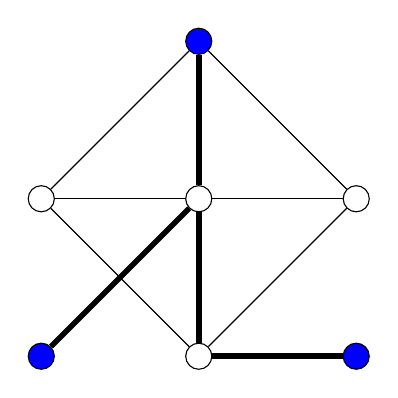
\begin{tikzpicture}[node distance={30mm}, main/.style = {draw, circle}] 
        \node[main, fill=blue] (1) at (2, 4) {}; 
        \node[main] (2) at (0, 2) {};
        \node[main] (3) at (2, 2) {};
        \node[main] (4) at (4, 2) {};
        \node[main, fill=blue] (5) at (0, 0) {};
        \node[main] (6) at (2, 0) {};
        \node[main, fill=blue] (7) at (4, 0) {};

        \draw (1) -- (2);
        \draw[line width=2pt] (1) -- (3);
        \draw (1) -- (4);
        \draw (2) -- (3);
        \draw (2) -- (6);
        \draw (3) -- (4);
        \draw[line width=2pt] (3) -- (5);
        \draw[line width=2pt] (3) -- (6);
        \draw (4) -- (6);
        \draw[line width=2pt] (6) -- (7);
    \end{tikzpicture} 
\end{center}
\vspace{-0.25cm}
Note that we have already seen some particular instances of this problem before.
\begin{itemize}
    \item If $T = \varnothing$, then this problem is trivial; just don't take any edges.
    \item If $|T| = 2$, then this is the shortest path problem.
    \item If $T = V$, then this is the minimum spanning tree problem.
\end{itemize}
However, it turns out that this problem is NP-hard in general!

\subsection{Minimum Metric Steiner Tree Problem} \label{subsec:5.2}
This problem is a minimum Steiner tree problem where we impose the additional 
conditions that
\begin{enumerate}[(a)]
    \item $G = (V, E)$ is complete; and 
    \item $c_{uw} \leq c_{uv} + c_{vw}$ for all distinct $u, v, w \in V$.
\end{enumerate}
Since the edge costs satisfy the triangle inequality, we are living 
in a metric space in some sense, which explains the name of the problem.

It turns out that these problems are equivalent, even though the metric 
version looks like a much more specific case than the original version! 
In our reluctance to call this the \textsc{MST} problem due to minimum 
spanning trees, let's call them \textsc{MSteinerT} and \textsc{MMSteinerT}
respectively. 

If we have an oracle for \textsc{MSteinerT}, then given an instance of 
\textsc{MMSteinerT}, we can simply feed it to the oracle for \textsc{MSteinerT}
as it solves the more general problem. The hard part of the equivalence 
is proving the other direction where if we have an oracle for 
\textsc{MMSteinerT}, then we can also solve \textsc{MSteinerT} efficiently.

Suppose we are given an instance of \textsc{MSteinerT} $(G, c, T)$, 
where $G = (V, E)$. Consider $(G', c', T')$, where
\begin{itemize}
    \item $T' = T$;
    \item $G' = (V, E')$ is the complete graph on the vertices of $G$; and 
    \item $c'_{uv}$ is the length of a shortest $u,v$-path in $G$ with 
    respect to edge costs $c_e$.
\end{itemize}
The following lemma tells us that $(G', c', T')$ is in fact an instance of 
\textsc{MMSteinerT}.

\begin{lemma}{lemma:5.1}
    \begin{enumerate}[(a)]
        \item For every Steiner tree $F$ for the instance 
        $(G, c, T)$, $F' = F$ is also a Steiner tree for the 
        instance $(G', c', T')$ of cost 
        $c'(F') \leq c(F)$. 
        \item For any Steiner tree $F'$ for the instance 
        $(G', c', T')$, there is a Steiner tree $F$ for the 
        instance $(G, c, T)$ such that $c(F) \leq c'(F')$. 
        \item The new edge costs $c'$ satisfy the triangle inequality. In particular, 
        $(G', c', T')$ is an instance of \textsc{MMSteinerT}.
    \end{enumerate}
\end{lemma}\vspace{-0.25cm}
\begin{pf}[Lemma~\ref{lemma:5.1}]
    \begin{enumerate}[(a)]
        \item Since $E' \supseteq E$, we have that $F \subseteq E'$. Moreover, 
        $F$ is still a tree and connects all vertices in $T = T'$. Note that 
        for every edge $e \in E$, we have $c'_e \leq c_e$ because 
        taking the edge $e = uv$ is among one possibility for a $u,v$-path
        and $c'_e$ corresponds to the length of the shortest one. This 
        gives us $c'(F) \leq c(F)$. 
        \item For each $uv \in F'$, consider a shortest $u, v$-path 
        $P_{uv}$ in the original instance $(G, c, T)$. Let 
        \[ K = \bigcup_{uv \in F'} P_{uv} \] 
        be the union of all the edges in these shortest paths. (Note that 
        $K$ is not necessarily a tree.) Since $c(P_{uv}) \leq c'_{uv}$ 
        by construction, we have 
        \[ c(K) \leq c'(F') = \sum_{uv \in F'} c'_{uv}. \]
        Also, $K$ consists only of edges in the original graph $G$ and 
        connects all terminals in $T$. Consider the subgraph  
        with $K$ as the edges and look at the connected component containing 
        the terminals in $T$. Construct a spanning tree $F$ on this connected 
        component. Then $c(F) \leq c(K) \leq c'(F')$ and $F$ connects 
        the terminals in $T$, so it is a Steiner tree for $(G, c, T)$. \qed
    \end{enumerate} 
\end{pf}\vspace{-0.25cm}